\section{使用集成工具获取鼠标光标的位置}

为了确保获取的坐标位置准确,\textbf{\color{red}必须}首先运行随附的工具(Tool 文件夹下的 \lstinline{Tool.exe},图 \ref{ch2fig-run-tool})将游戏窗口居中。

\begin{figure}[H]
    \Centering
    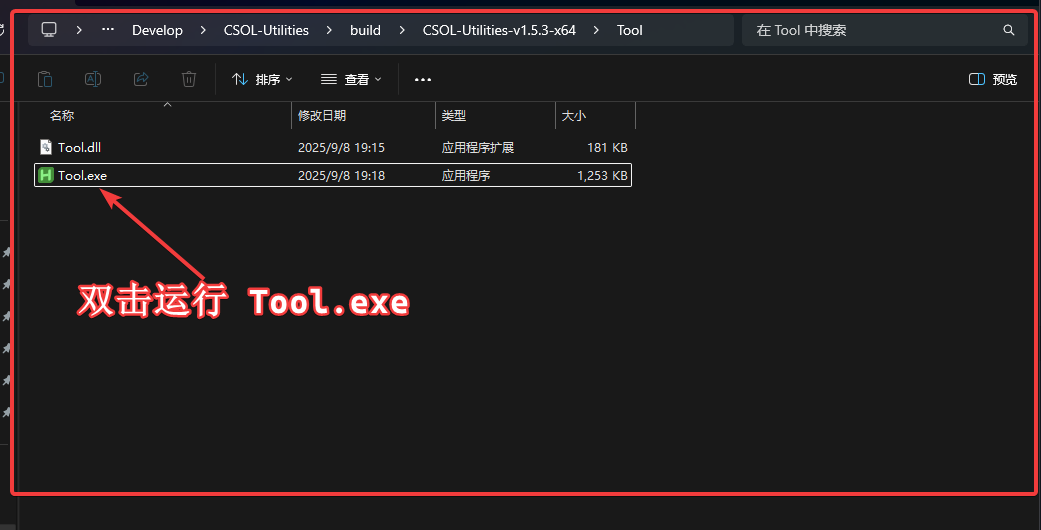
\includegraphics[width=\textwidth]{assets/run_tool.png}
    \caption{打开 Tool.exe}
    \label{ch2fig-run-tool}
\end{figure}

双击运行工具后,激活游戏窗口,按下 \lstinline{Ctrl} \lstinline{Alt} \lstinline{C} 即可将游戏窗口居中,挂机时不强制要求开启 Tool(控制器会自动居中窗口)。有关 \lstinline{Tool.exe} 的更多信息请参阅使用手册。
居中前后对比效果如下:
    
\begin{figure}[H]
    \Centering
    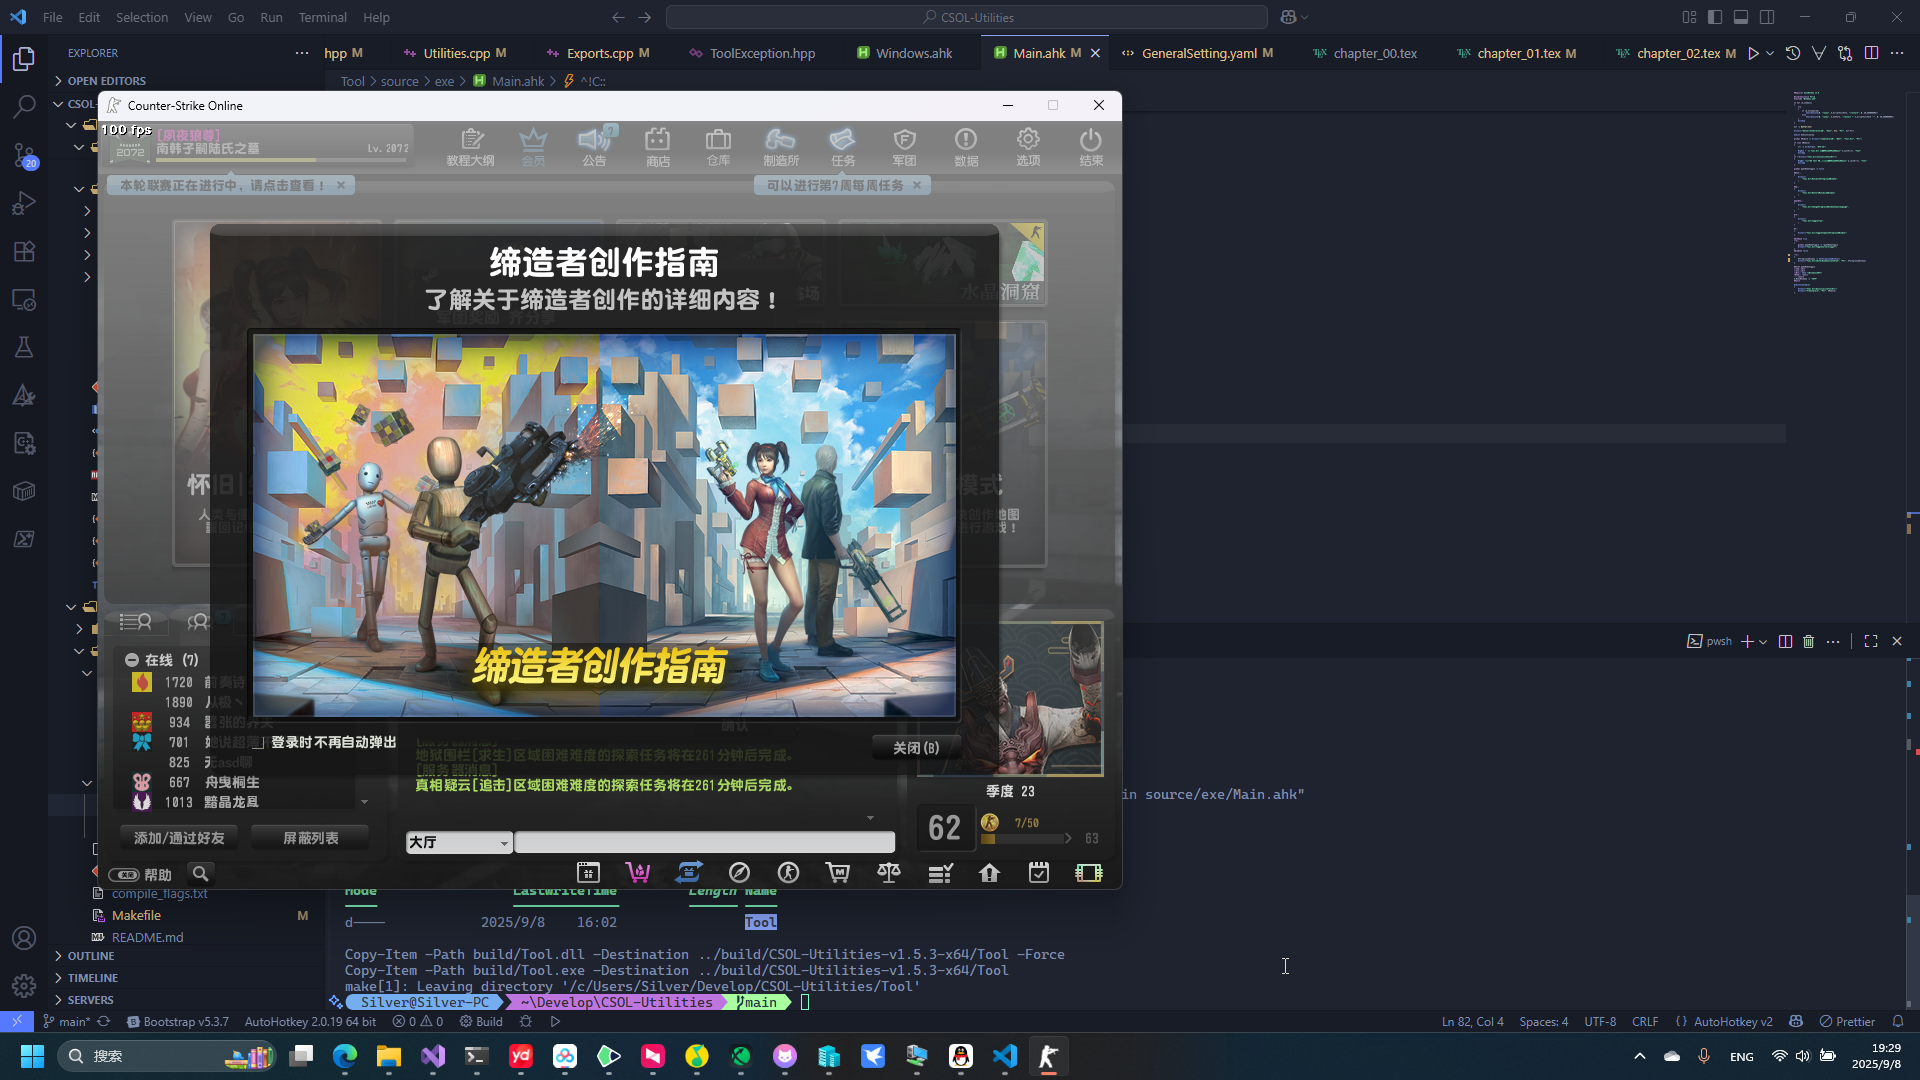
\includegraphics[width=\textwidth]{assets/before_center.png}
    \caption{居中前}
    \label{ch2fig-before-center}
\end{figure}

\begin{figure}[H]
    \Centering
    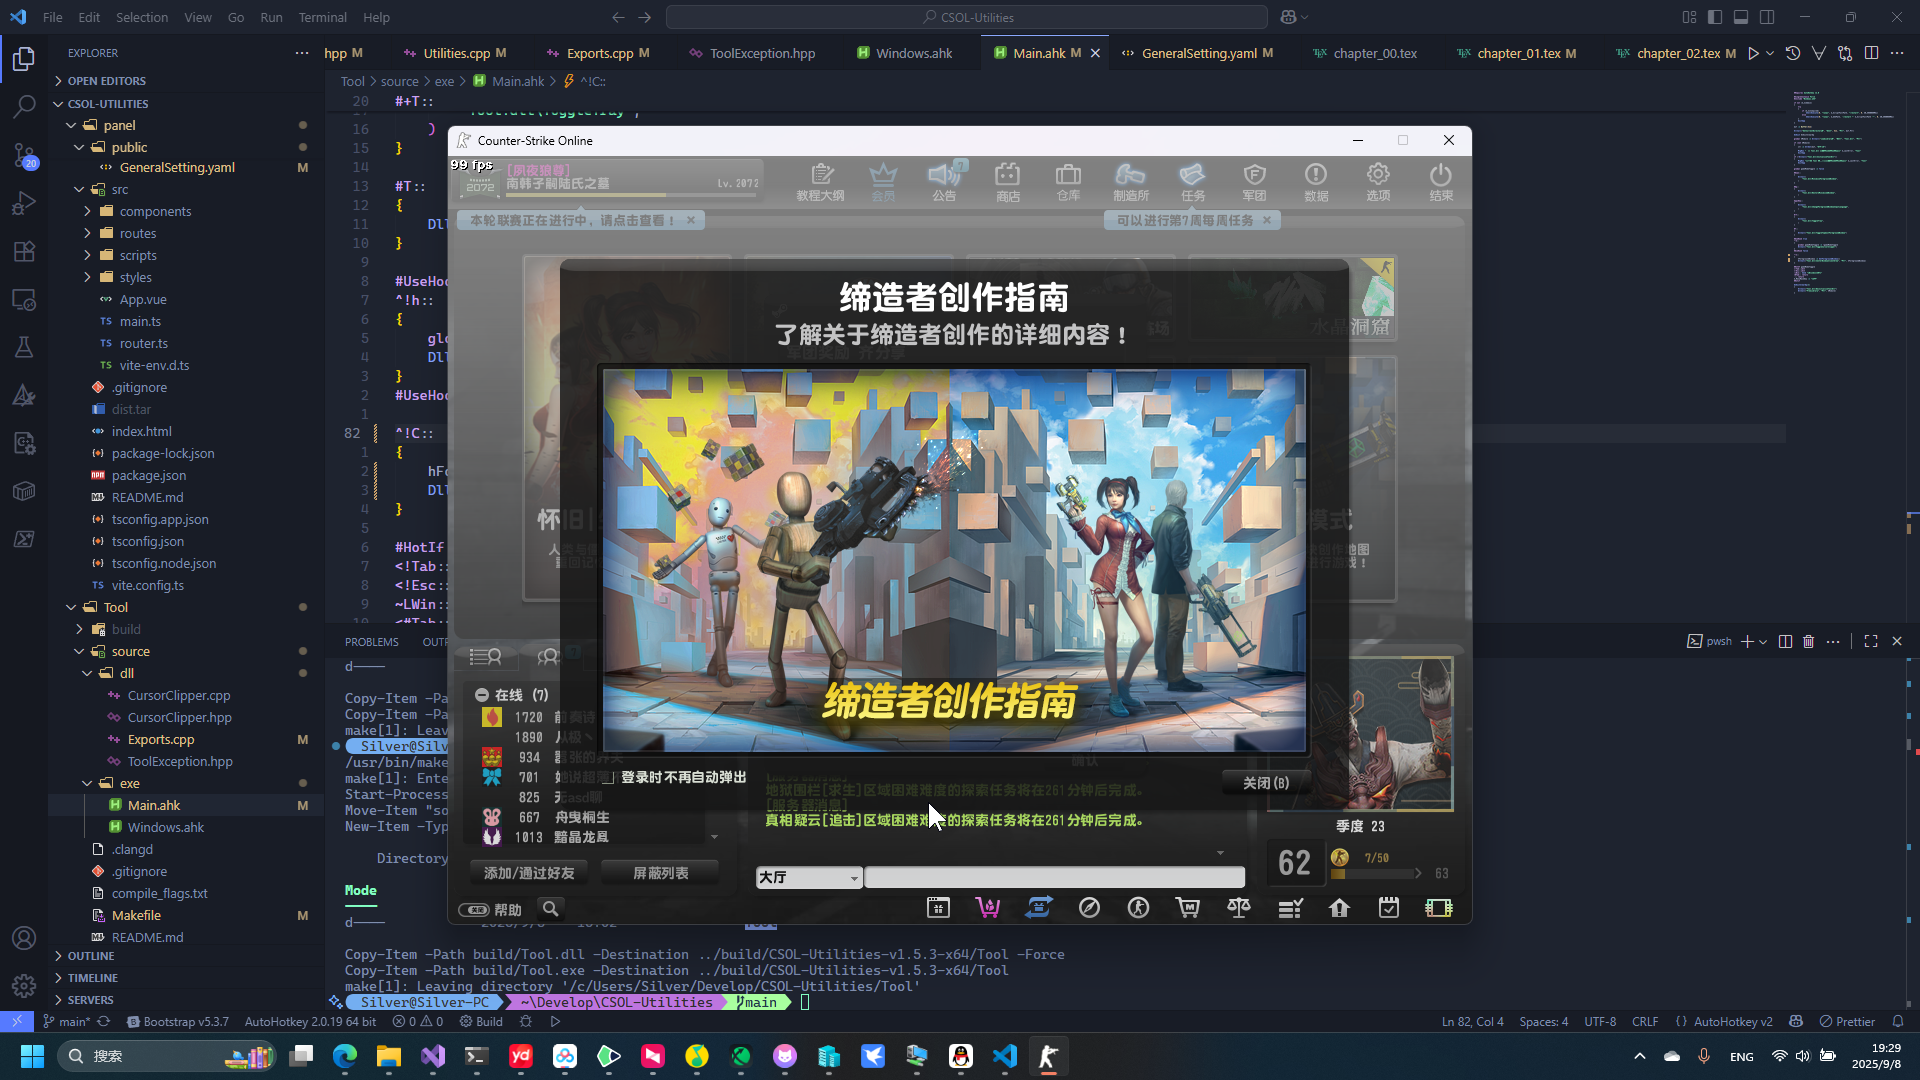
\includegraphics[width=\textwidth]{assets/after_center.png}
    \caption{居中后}
    \label{ch2fig-after-center}
\end{figure}

要退出 Tool.exe,在任务栏找到下面的图标,右键后点击“Exit”退出。

控制器运行后,按下 \lstinline{Ctrl} \lstinline{Alt} \lstinline{Shift} \lstinline{5},将集成工具切换到 5 模式进行光标定位。

\begin{figure}[H]
    \Centering
    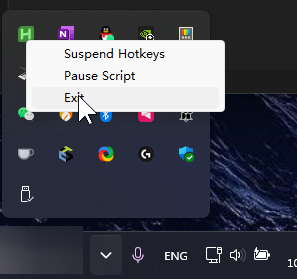
\includegraphics[width=\textwidth]{assets/exit_tool.png}
    \caption{退出 Tool.exe}
\end{figure}

将鼠标光标移动到欲确定坐标的位置后,\textbf{\color{red}同时按下 \lstinline{Ctrl} 和 \lstinline{Alt}},罗技控制台中将输出鼠标光标的坐标位置。

\begin{figure}[H]
    \Centering
    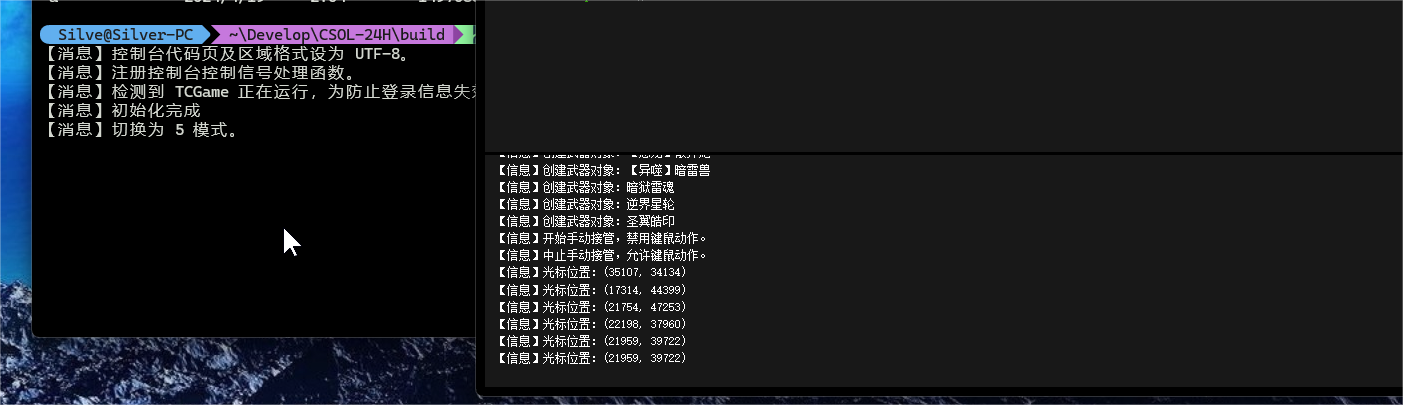
\includegraphics[width=\textwidth]{assets/position.png}
    \caption{获取鼠标光标位置}
\end{figure}